\documentclass[shortdoc,ngerman,numberall]{article}
\usepackage{babel}  
\usepackage{siunitx}  
\sisetup{locale = DE}
\usepackage { tabularx }
\usepackage{graphicx}
\usepackage{caption}
\captionsetup[figure]{labelformat=empty}
\usepackage{pgfplots}
\usepackage{lmodern}
\usepackage{floatflt}
\usepackage{float}
\usepackage{wrapfig}
%\usepackage{subfigure}

\pgfplotsset{compat=newest}
\pgfplotsset{plot coordinates/math parser=false}
\newlength\figureheight
\newlength\figurewidth
%\usetikzlibrary{arrows,shapes,calc, positioning, patterns, decorations, decorations.markings}
\usepackage{forest}
%\usepackage{float}
%\setbeamercovered{transparent}
\usepackage[flushleft]{threeparttable}
%\floatstyle{plaintop}
%\usepackage{url}
\usepackage{booktabs}
\usepackage{siunitx}
\usepackage{url}
%\linespread{1.5}
\usepackage{setspace}
\usepackage[siunitx,european]{circuitikz}
\usepackage{multicol}

\usepackage[hang]{footmisc} %Gleichmäßiger Einzug der Fußnoten
\setlength{\footnotemargin}{-0.8em}
\usepackage{tikz}
\usepackage{graphicx}



\usepackage{caption}
\usepackage{subcaption}

\usepackage{mathtools}
\usepackage{amsmath}
\usepackage{mathptmx} % Use the Times font for serif text
\usepackage{palatino} % Use the Palatino font for serif text
\usepackage{adjustbox}
\usepackage{resizegather}

\begin{document}{\fontfamily{phv}\selectfont
	
	\section*{ Mathematische Modellierung}
Es gibt mehrere Methoden, um den Doppelpendel zu modellieren. In diesem Zuge bietet der Lagrange-Formalismus die Möglichkeit, die Bewegungsgleichungen bei komplizierten mechanischen Systemen aufzustellen. Unter Betrachtung der Bezugskoordinaten an der Stelle $\boldsymbol{O}$ hat das Modell Doppelpendel zwei unabhängige verallgemeinerte Koordinaten, die Auslenkung des ersten Pendels $\theta_1$ und des zweiten Pendels $\theta_2$.\\


\begin{figure}[!h]
	\centering
	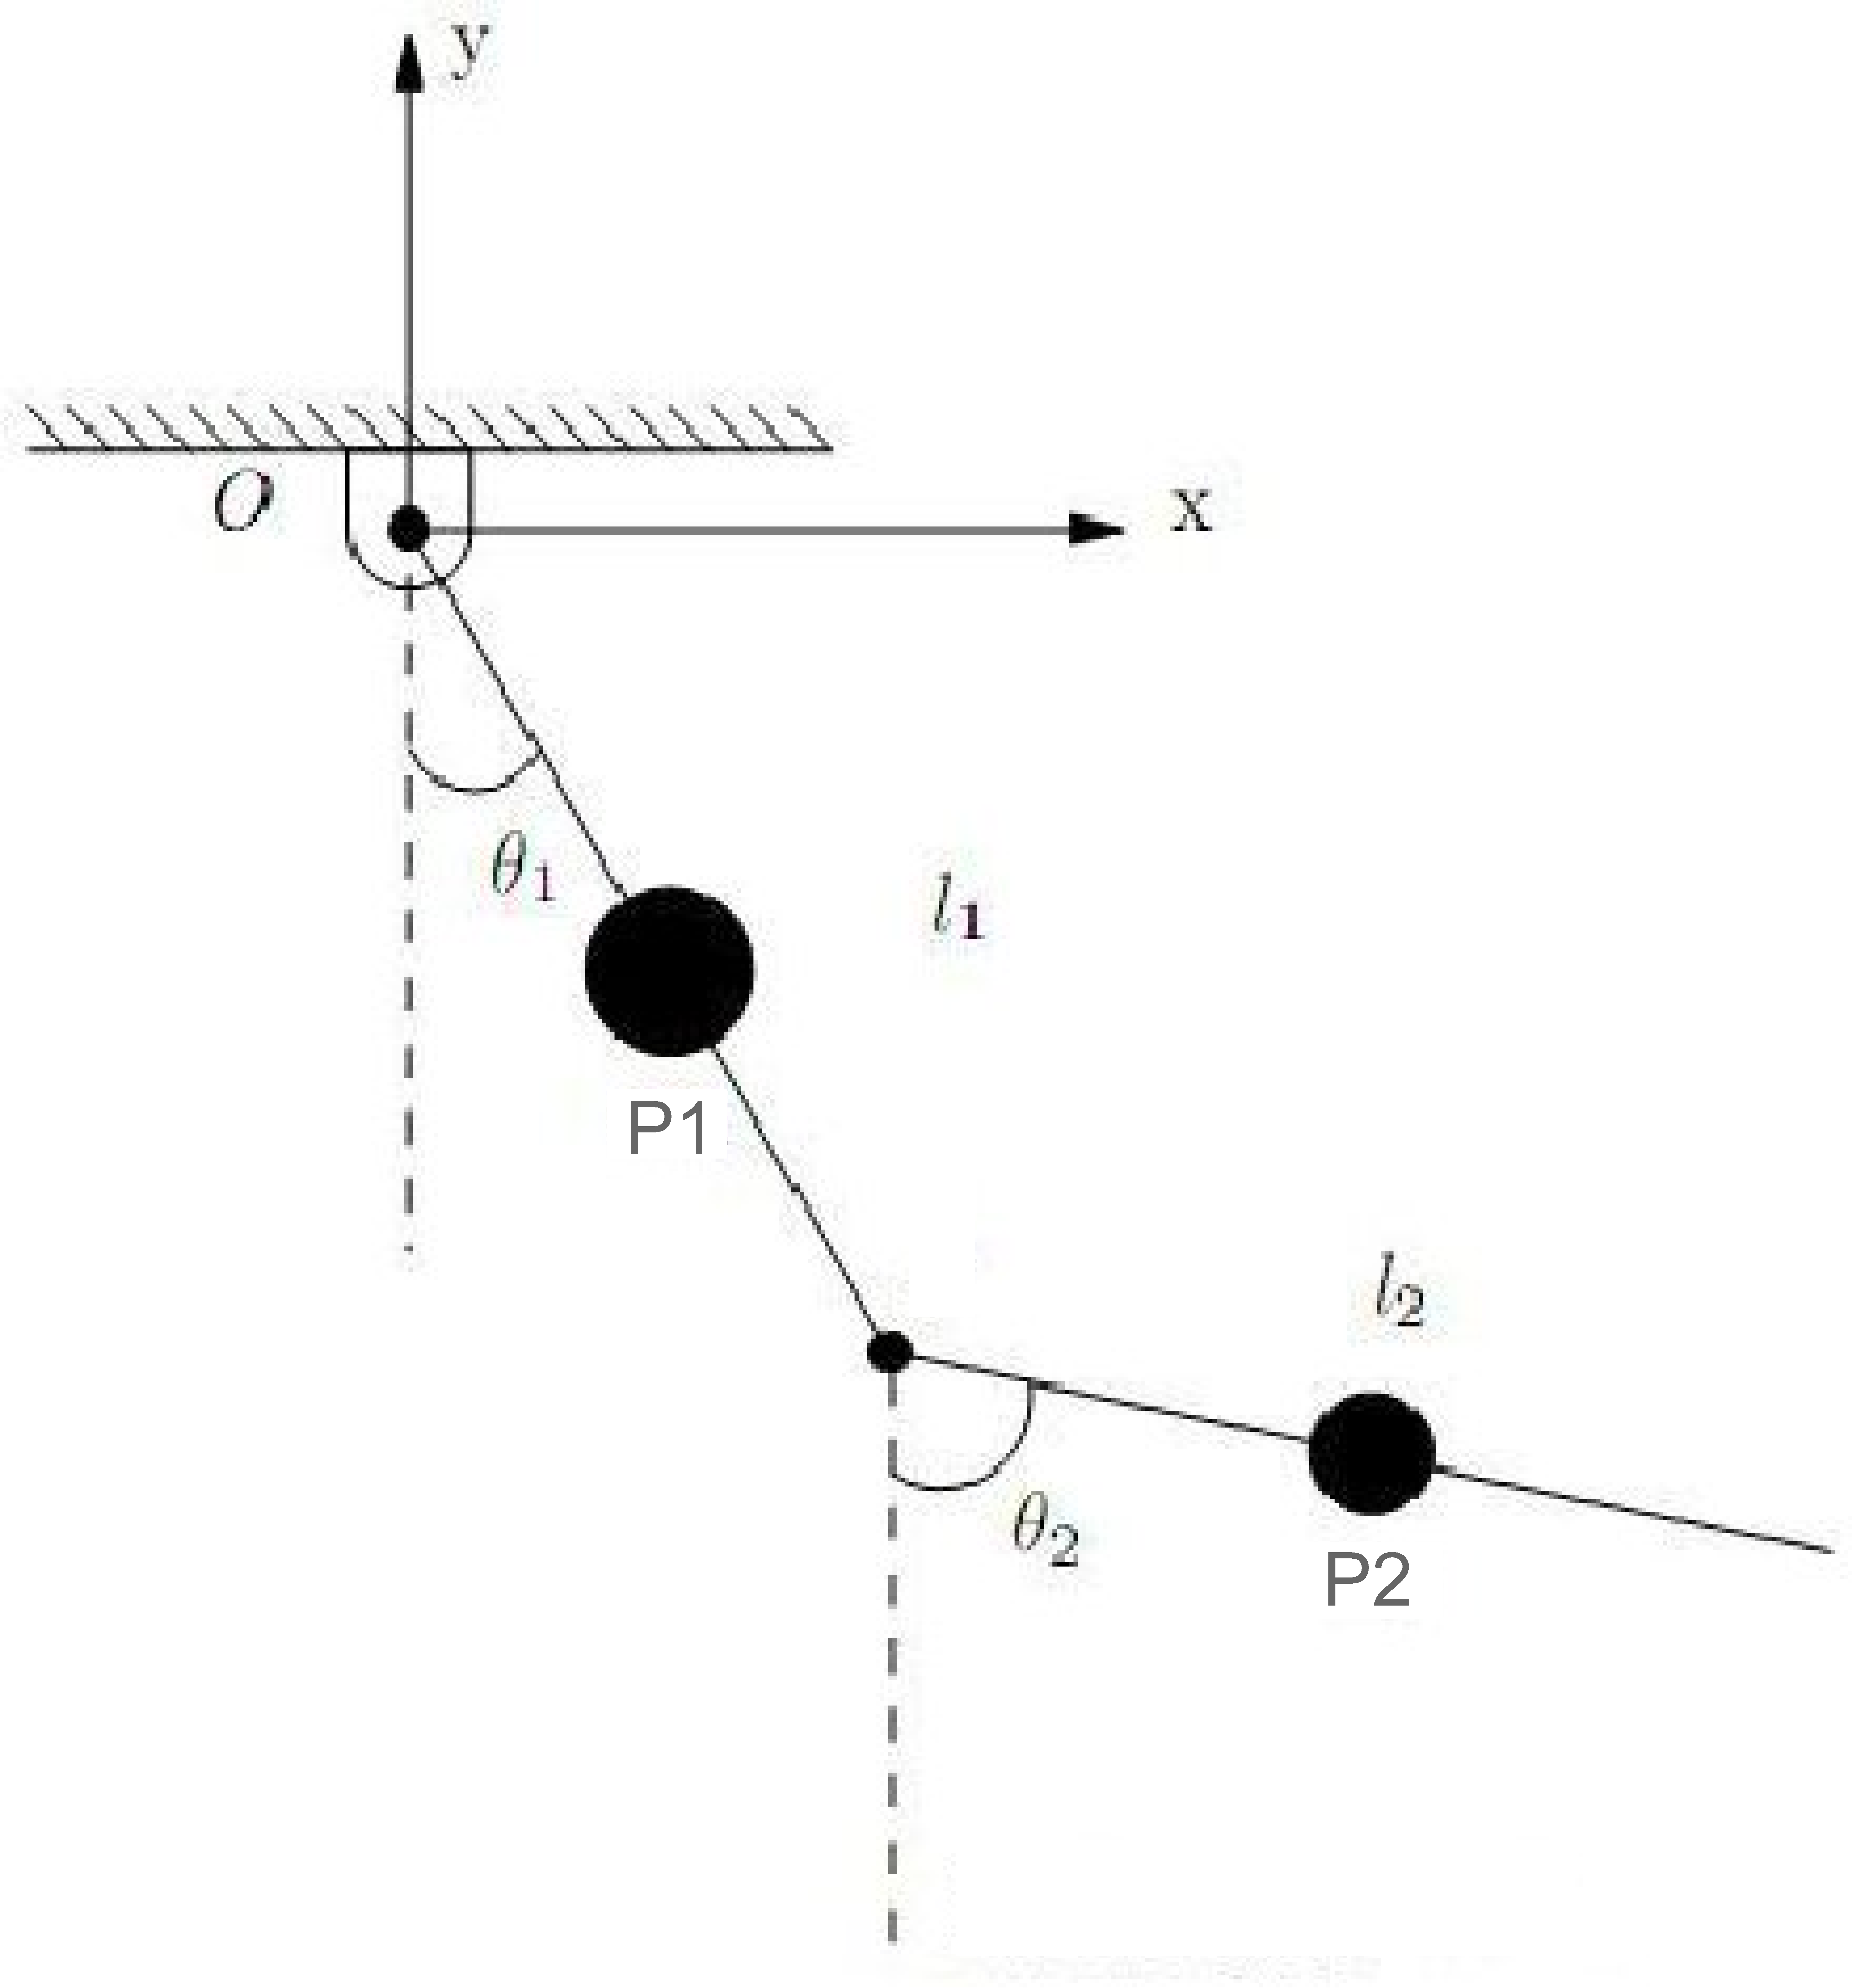
\includegraphics [scale=0.065]{Doppelpendel.pdf}
	%   \vspace{-2 mm}
	\caption{Ersatzschlatbild des Doppelpendels}
	\label{Doppelpendel}
\end{figure}
Die Lagrange-Funktion wird als:\\
\begin{align*}
	L&= K-U,\\
	K&=\frac{1}{2} ( m_1 v_1^2 + m_2 v_2^2 + I_1 \theta_1^2+ I_2 \theta_2^2)\\
	U&= m_1 g y_1 + m_2 y_2
\end{align*}
Die Euler-Lagrange-Gleichung lautet

\begin{align*}
	\frac{\text{d}}{\text{d}t} \frac{\partial L}{\partial \dot{q_{i}}}- \frac{\partial L}{\partial q_{i} } = 0,  \quad  \text{Mit} \quad q_i = \theta_i , \quad i =1,2.
\end{align*}
}
\end{document}